




As noted in the previous section, the k-d tree build process is by far the most expensive operation, and we would save a lot of time by managing to parallelize it. This introduces a new resource question.

\begin{myrq}
\label{rq:parallel_build}
    It is possible to parallelize the k-d tree build algorithm, in such a way that it gives a significant speed improvement compared to the serial algorithm.
\end{myrq}

In order to investigate this RQ, we have to look a bit closer at the different steps of the k-d tree build algorithm and look at different parallelization strategies.

Steps:
\begin{enumerate}
    \item Find the median of the points along a specified axis. This median point becomes the value of the current node.
    \item Sort all points with lower values than the median to the left of the median, and all the points with higher values than the median to the right.
    \item Perform this algorithm recursively on the left and right set of nodes.
\end{enumerate}

If we analyze the algorithm \ref{alg:seriel_tree_build}, we can see that for each node in the k-d tree a median finding and a partition has to be made, as described in step 1 and 2. We can call this recursive step a node task. This node task has to be done for all nodes starting at the root and successively go down the tree.


\subsubsection{Parallelization strategy} % (fold)
\label{ssub:parallelization_strategy}


First a good overall parallelization strategy has to be found. A good strategy manage to easily split the main task into small individual subtasks. From the serial recursive algorithm \ref{alg:seriel_tree_build}, we see that there are two recursive calls. This is logical, because we are building a binary tree.  The interesting observation is that a node task is only dependent on the parent node tasks. This means that each tree level are independent, which acts as a good start for our parallelization strategy.

Some other small observation, in regard of a parallelization strategy, is that all subtrees in the k-d tree generation are independent. Hence, the tree corresponding to the left and right child of a node can be done in parallel without any communication. The data is also independent, as a result of how we represent the tree as an array. By data independent, it is meant that the data structure easily can be partitioned to each subtask. In our case will the tree array successively be partitioned into contentious sublists, one for each node task.

From these observations, several strategies can be used to parallelize the k-d tree build algorithm. From the first observation a trivial strategy is to divide the tree levels into dependent tasks, where each node task in a tree level is a independent subtask. This gives us an power of two increasing number of parallel nodes tasks as we increase the tree level. The sublist size will decrease with a factor of two in each downward step. An other strategy is to parallelize each node task.

Both strategies can be used in conjunction with each other. The parallel node task algorithm can be used to speed up the early iterations, where the amount of node task in a tree level is small. As well as further parallelize the subtasks in later tree level iterations.

% subsubsection parallelization_strategy (end)


% TODO: Header must be improved
\subsubsection{Selecting an algorithm} % (fold)
\label{ssub:selecting_a_algorithm}



As we have seen in section \ref{sub:application_of_kd_trees_to_the_knn_problem}, many algorithms for finding median exist. Since we now want to implement the algorithm with CUDA, the environment has changed, and quick select may not be the best alternative anymore. The first problem with quick select is that it is recursive, which makes it hard to parallelize on CUDA. This is because in a recursive implementation the programs institution and control flow is hided in the threads call stack, and not accessible to the other threads. We therefor have to find an other algorithm, which is easier to parallelize.


First we tried to reuse the implementation of bitonic sort. Given a sorted list you can find the median directly, by simply looking at the midmost element of the array. The partitioning is also done in the process. Unfortunately this strategy proved unsuccessful, as re-purposing the bitonic algorithm for such an task proved difficult. The reason for this is that a pure bitonic sort only manage to sort lists with a length of power of two. The normal solution is to create a longer list then needed, which destroys many of the advantages with our binary tree representation. There are also some other solutions to the problem, for example one by K.E. Batcher \cite{Batcher:1968}, but these solutions introduces a lot of divergence that destroys performance on the GPU. We also have the inherent downside of sorting a list in order to find the median, since \BigO{n} algorithms for finding the median exist, compared to the \BigO{n log(n)} time required by sorting.


The existing linear algorithms for finding the median is mostly based on a more generic problem, namely selection or k'th order statistic algorithms \citep{Cormen:2001}. Our serial choice, Quick select, is one of these. It is possible to implement a iterative version, so that the bad properties from the recursive version are eliminated. This option is ignored, because, literature states that there are other better suited algorithms, like Alabi \citep{Alabi:2012}. Alabi goes through the radix select and bucket select algorithm in detail. The difference between them is the constant time penalty. The radix sort have a more exact time complexity of \BigO{bn}, where b is the number of bits in each number. While the penalty for bucket select is \BigO{an}, where $a$ stands for the degree of adversarial in the values. The algorithm is week when the points is clusters together. His results shows that bucket select normally is slightly faster, except when $a$ is high. Although bucket select normally have better results, we choose radix select. The reason is that we expect high degree of adversarial in our application.


\subsubsection{Radix select} % (fold)
\label{ssub:radix_select}

% subsubsection radix_select (end)

The radix select is based on a bitwise partitioning, much like radix sort. In each step, elements are partitioned in two subgroups based on the current bit. Then the subgroup that contains the median is determined, and the search continue in that subgroup until the median is found.

\begin{figure}[ht!]
\centering
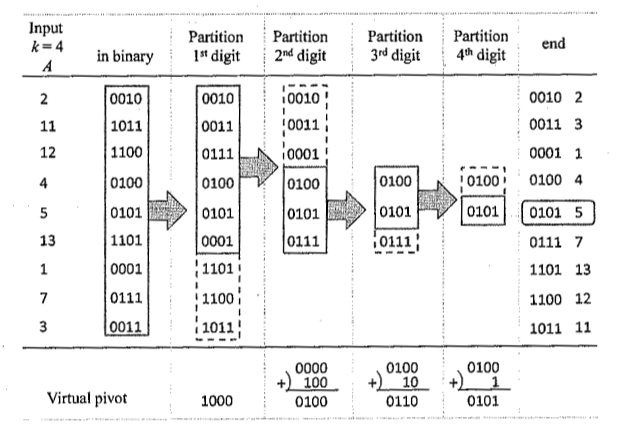
\includegraphics[width=100mm]{../gfx/Radix_select.png}

\caption{An illustration of radix selection \cite{cayman:2012}.}
\label{fig:radix_select}
\end{figure}






% It is hard to use all the parallel power of cuda in this algorithm. The reason is that the problem is divided in three different types; partition one huge list, partition some middle sized list and partition many small lists. This is the reason why we have chosen to use three different implementation of k'th order statistic. The constant time penalties of the two algorithms we have chosen give us a clear indication the radix select is best on large lists while quick select is best on small lists.

% Results:
% \begin{figure}[ht!]
% \centering
% 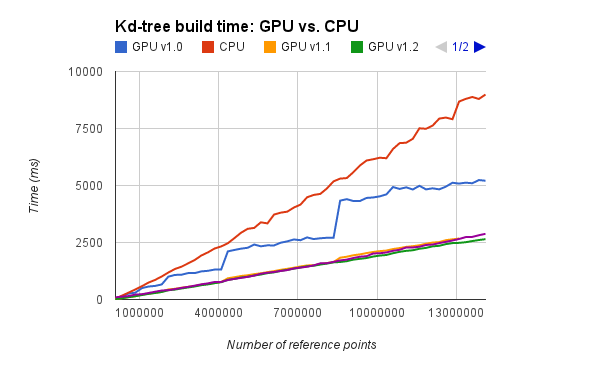
\includegraphics[width=120mm]{../gfx/gpu-vs-cpu-build-time.png}

% \caption{GPU vs CPU build time.}
% \label{fig:sublime_ide}
% \end{figure}

% We see that the parallel implementation performs better than the base serial implementation, building a tree of 14 million points in just over 5 seconds, compared to just under 10 required by the serial algorithm. Still we regard this as a quite rough implementation, in need of more tuning to really bring out the speed potential. The potential for parallelizing the workload for the first and last iterations have not been fully developed. This is due to the implementation forcing one version of the radix select algorithm being to work on all problem sizes. This is not optimal for dividing cuda resources, and as a result, we get high penalties when the problem size reaches unsuitable values.

% We also see a couple of large jumps in the graph. This happens when the number of elements passes a power of two and the height of the resulting k-d tree increase. The height increase hits the implementation at its weakest.

% Tuning the algorithm to alternate between radix select and quick select, eliminates this problem, as is visible in the graph for GPU v1.1. This removes the penalty for calculating the median at unsuitable problem sizes, giving an build time of ~2.4 seconds for 14 million points, compared to the ~9 seconds required by the serial implementation, or the ~5.2 seconds required by the old parallel implementation.

% % subsubsection selecting_a_algorithm (end)
% Memory usage:

% To analyses the space complexity of the k-d tree build and search algorithm, we have made an theoretical calculation of both algorithms GPU memory consumption, and tested it against results from a GeForce 560ti and a Nvidia grid K520 (amazon web service delved).

% It is important to note that the only hard memory limitation is related to building the tree, as a search for N query-points can be performed in several operations. If you e.g. run into memory limitations when searching for pow(10, 8) query-points, you can simply perform two searches on pow(5, 8) query-points to get around the limitation. Loading the pre-built k-d tree on the GPU for searching, and performing one query for a low value of k, will always consume less memory than building the actual k-d tree.

% **Kd-tree-build**

% The memory consumption for the k-d tree build is only depended on the number of points (n) and the theoretical consumption rate grows linearly as \BigO{36n} subset of \BigO{n}.

% \begin{figure}[ht!]
% \centering
% 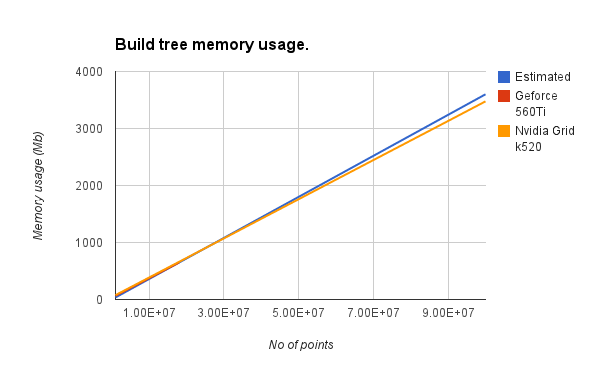
\includegraphics[width=120mm]{../gfx/memory-usage-build.png}

% \caption{Memory usage of k-d tree-build.}
% \label{fig:memory_usage_build}
% \end{figure}

% We see that the estimation fit the real consumption almost perfectly, and with this memory model, we can easily estimate the GPU memory requirements for different problem sizes.

% Given that a customer wants to perform a knn-search on a point cloud of 100 million, he or she would need a GPU with at least 3.6 Gb of spare memory. Under we have tabulated what maximum problem sizes you would expect to be able to run on a selection of Nvidia graphics cards:

% \begin{center}
%     \begin{tabular}{ | l | l | p{5cm} |}
%     \hline
%     Nvidia GPU & Available memory & Maximum problem size \\ \hline
%     GTX TITAN & 6144 MB & 1.79E+08 \\ \hline
%     GTX 780 & 3072 MB & 8.95E+07 \\ \hline
%     GTX 770 & 2048 MB & 5.97E+07 \\ \hline
%     Quadro K6000 & 12288 MB & 3.58E+08 \\ \hline
%     Quadro K5000 & 4096 MB & 1.19E+08 \\ \hline
%     Quadro K4000 & 3072 MB & 8.95E+07 \\ \hline
%     Tesla K40 & 12288 MB & 3.58E+08 \\ \hline
%     Tesla K20 & 5120 MB & 1.49E+08 \\ \hline
%     \end{tabular}
% \end{center}

% These numbers should be read as rough estimates, as each card is expected to have internal processes requiring an unspecified constant amount of the available memory, therefor lovering the maximum problem size possible to run on these cards in practice. It is also worth to mention that when buying a GPU for GPGPU tasks, other performance characteristics is equally, or more, important.

% **Kd-search**

% The kd-search is used to query every point against each other. It has a theoretical memory consumption rate at \BigO({40+4k}n) subset of \BigO{kn}. The consumption is therefore depended on the number of points (n) and the number of neighbors (k).

% \begin{figure}[ht!]
% \centering
% 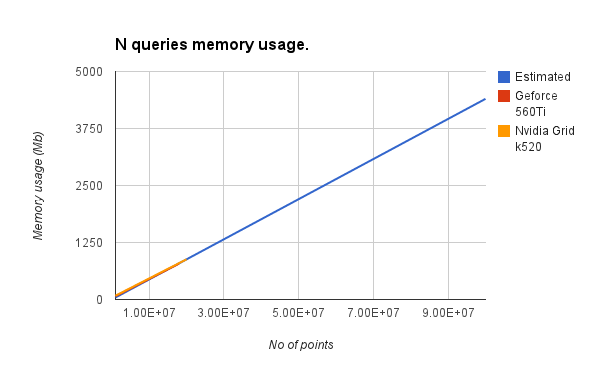
\includegraphics[width=120mm]{../gfx/memory-usage-kd-search.png}

% \caption{Memory usage of kd-search.}
% \label{fig:memory-usage-kd-search}
% \end{figure}

% Also in this case our estimation fit the real consumption with a high degree of accuracy.

% Further work:
% \begin{itemize}
%     \item Look at memory optimization.
%     \item Improve utiliti methods like: accumulateindex, minReduce.
%     \item Forloop Unrolling.
% \end{itemize}
